\documentclass{beamer}

\usepackage{amsmath}

\usetheme{AnnArbor}
\usecolortheme{crane}
\usefonttheme[onlymath]{serif}

\title{Deep Learning - Foundations and Concepts}
\subtitle{Chapter 5. Single-layer Networks: Classification}
\author{nonlineark@github}
\date{\today}

\begin{document}

\begin{frame}
    \titlepage
\end{frame}

\begin{frame}
    \frametitle{Outline}
    \tableofcontents
\end{frame}

\section{Discriminant Functions}

\begin{frame}
    \frametitle{Discriminant functions}
    \begin{itemize}
        \item The goal in classification is to take an input vector $x\in\mathbb{R}^{D}$ and assign it to one of $K$ discrete classes $\mathcal{C}_{k}$.
        \item A discriminant is a function that takes an input vector $x$ and assigns it to one of $K$ classes, denoted $\mathcal{C}_{k}$.
        \item We will restrict attention to linear discriminants, for which the decision surfaces are hyperplaines.
    \end{itemize}
\end{frame}

\begin{frame}
    \frametitle{Two classes}
    Taking a linear function of the input vector:
    \begin{equation*}
        y(x)=w^{T}x+w_{0}
    \end{equation*}
    \begin{itemize}
        \item An input vector is assigned to class $\mathcal{C}_{1}$ if $y(x)\ge{}0$ and to class $\mathcal{C}_{2}$ otherwise.
        \item The decision boundary is a $(D-1)$-dimensional hyperplane.
    \end{itemize}
\end{frame}

\begin{frame}
    \frametitle{Two classes}
    \begin{figure}
        \caption{The geometry of a linear discriminant function in two dimensions}
        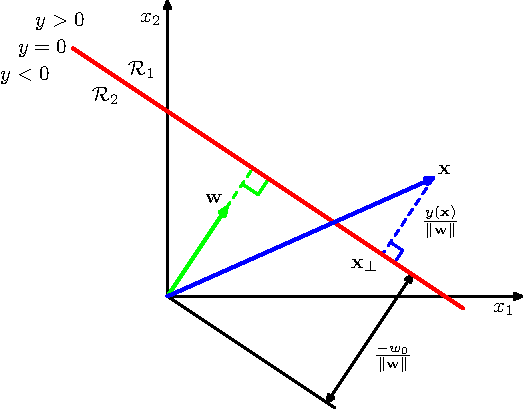
\includegraphics[height=0.6\textheight]{Figure_1.pdf}
    \end{figure}
\end{frame}

\begin{frame}
    \frametitle{Two classes}
    It's easy to see that:
    \begin{itemize}
        \item $w$ is orthogonal to the decision surface.
        \item $w$ points to the direction of the increase of $y$.
    \end{itemize}
    Also the value of $y(x)$ gives a signed measure of the perpendicular distance $r$ of the point $x$ from the decision surface:
    \begin{align*}
        x&=x_{\perp}+r\frac{w}{||w||} \\
        y(x)&=w^{T}x+w_{0}=w^{T}x_{\perp}+w_{0}+r||w||=r||w|| \\
        r&=\frac{y(x)}{||w||}
    \end{align*}
    In particular, the signed distance of the origin from the decision surface is given by $\frac{w_{0}}{||w||}$.
\end{frame}

\begin{frame}
    \frametitle{Multiple classes}
    Building a $K$-class discriminant by combining a number of two-class discriminant functions usually doens't work:
    \begin{itemize}
        \item One-versus-the-rest.
        \item One-versus-one.
    \end{itemize}
\end{frame}

\begin{frame}
    \frametitle{Multiple classes}
    Consider a single $K$-class discriminant comprising $K$ linear functions of the form:
    \begin{equation*}
        y_k(x)=w_{k}^{T}x+w_{k0}
    \end{equation*}
    Assign a point $x$ to class $\mathcal{C}_{k}$ if $y_k(x)>y_j(x)$ for all $j\ne{}k$. The decision boundary between class $\mathcal{C}_{k}$ and $\mathcal{C}_{j}$ is given by $y_k(x)=y_j(x)$ and corresponds to a $(D-1)$-dimensional hyperplane:
    \begin{equation*}
        (w_{k}-w_{j})^{T}x+(w_{k0}-w_{j0})=0
    \end{equation*}
    The decision regions of such a discriminant are always singly connected and convex.
\end{frame}

\begin{frame}
    \frametitle{Multiple classes}
    \begin{figure}
        \caption{The decision regions for a multi-class linear discriminant}
        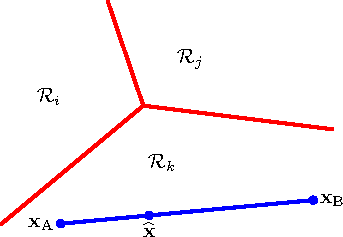
\includegraphics{Figure_3.pdf}
    \end{figure}
\end{frame}

\begin{frame}
    \frametitle{Linear squares for classification}
    Consider a general classification problem with $K$ classes:
    \begin{itemize}
        \item There are $N$ input data: $x^{1},\hdots,x^{N}$, where $x^{n}\in\mathbb{R}^{D}$.
        \item There are $N$ target data: $t^{1},\hdots,t^{N}$ using a $1$-of-$K$ binary coding scheme, thus $t^{n}\in\mathbb{R}^{K}$.
        \begin{itemize}
            \item Let $T=\begin{pmatrix}
                t^{1}&t^{2}&\hdots&t^{N}
            \end{pmatrix}^{T}\in\mathbb{R}^{N\times{}K}$.
        \end{itemize}
        \item Each class $\mathcal{C}_{k}$ is described by its own linear model so that $y_k(x)=w_{k}^{T}x+w_{k0}$.
        \begin{itemize}
            \item Let $\tilde{w}_{k}=\begin{pmatrix}
                w_{k0} \\
                w_{k}
            \end{pmatrix}$ and $\tilde{W}=\begin{pmatrix}
                \tilde{w}_{1}&\tilde{w}_{2}&\hdots&\tilde{w}_{K}
            \end{pmatrix}\in\mathbb{R}^{(D+1)\times{}K}$.
            \item Let $\tilde{x}=\begin{pmatrix}
                1 \\
                x
            \end{pmatrix}$ and $\tilde{X}=\begin{pmatrix}
                \tilde{x}^{1}&\tilde{x}^{2}&\hdots&\tilde{x}^{N}
            \end{pmatrix}^{T}\in\mathbb{R}^{N\times(D+1)}$.
            \item Then $y_k(x)=\tilde{w}_{k}^{T}\tilde{x}$ and $y(x)=\tilde{W}^{T}\tilde{x}$.
        \end{itemize}
    \end{itemize}
\end{frame}

\begin{frame}
    \frametitle{Linear squares for classification}
    Let's determine the parameter matrix $\tilde{W}$ by minimizing a sum-of-squares error function:
    \begin{align*}
        E_{D}(\tilde{W})&=\frac{1}{2}\sum_{i,j}(\tilde{X}\tilde{W}-T)_{ij}^{2} \\
        &=\frac{1}{2}\mathrm{tr}((\tilde{X}\tilde{W}-T)^{T}(\tilde{X}\tilde{W}-T)) \\
        DE_{D}(\tilde{W})H&=\mathrm{tr}((\tilde{X}\tilde{W}-T)^{T}\tilde{X}H) \\
        \tilde{W}_{*}&=(\tilde{X}^{T}\tilde{X})^{-1}\tilde{X}^{T}T
    \end{align*}
\end{frame}

\begin{frame}
    \frametitle{Linear squares for classification}
    What property does $y(x)=\tilde{W}_{*}^{T}\tilde{x}$ has? Because $t^{n}$ is using a $1$-of-$K$ binary coding scheme, we know:
    \begin{equation*}
        \begin{pmatrix}
            1&1&\hdots&1
        \end{pmatrix}t^{n}=1
    \end{equation*}
    Thus we have:
    \begin{align*}
        \begin{pmatrix}
            1&1&\hdots&1
        \end{pmatrix}y(x)&=
        \begin{pmatrix}
            1&1&\hdots&1
        \end{pmatrix}\tilde{W}_{*}^{T}\tilde{x} \\
        &=\begin{pmatrix}
            1&1&\hdots&1
        \end{pmatrix}T^{T}\tilde{X}(\tilde{X}^T\tilde{X})^{-1}\tilde{x} \\
        &=\begin{pmatrix}
            1&1&\hdots&1
        \end{pmatrix}\tilde{X}(\tilde{X}^T\tilde{X})^{-1}\tilde{x} \\
        &=\mathrm{e}_{1}^{T}\tilde{X}^{T}\tilde{X}(\tilde{X}^{T}\tilde{X})^{-1}\tilde{x}=\mathrm{e}_{1}^{T}\tilde{x}=1
    \end{align*}
    That is, the predictions made by the model will have the property that the elements of $y(x)$ will sum to $1$ for any value of $x$.
\end{frame}

\begin{frame}
    \frametitle{Linear squares for classification}
    \begin{itemize}
        \item The model outputs cannot be interpreted as probabilities because they are not contrained to lie within the interval $(0,1)$.
        \item If the true distribution of the data is markedly different from being Gaussian, the least squares can give poor results.
        \item Least squares is very sensitive to the presence of outliers (a.k.a., lack robustness).
    \end{itemize}
\end{frame}

\section{Decision Theory}

\begin{frame}
    \frametitle{Misclassification rate}
    To minimize the chance of assigning $x$ to the wrong class, intuitively we would choose the class having the higher posterior probability.
    \begin{itemize}
        \item Divide the input space into regions $\mathcal{R}_{k}$ called decision regions.
        \item All points in $\mathcal{R}_{k}$ are assigned to class $\mathcal{C}_{k}$.
    \end{itemize}
    We want to maximize the probability of being correct:
    \begin{equation*}
        p(\textrm{correct})=\sum_{k=1}^{K}p(x\in\mathcal{R}_{k},\mathcal{C}_{k})=\sum_{k=1}^{K}\int_{\mathcal{R}_{k}}p(\mathcal{C}_{k}|x)p(x)\mathrm{d}x
    \end{equation*}
    It's easy to see that this is maximized when the regions $\mathcal{R}_{k}$ are chosen such that each $x$ is assigned to the class for which $p(\mathcal{C}_{k}|x)$ is largest. So the intuition is indeed correct.
\end{frame}

\begin{frame}
    \frametitle{Expected loss}
    \begin{itemize}
        \item Sometimes, our objective will be more complex than minimizing the number of misclassifications.
        \item We can introduce a loss function which measure loss incurred in taking any of the available decisions or actions and minimize the total loss.
    \end{itemize}
    If the true class for $x$ is $\mathcal{C}_{k}$ and we assign $x$ to $\mathcal{C}_{j}$, we incur some level of loss denoted by $L_{kj}$. Because we do not know the true class, instead of minimizing the loss function, we minimize its average:
    \begin{equation*}
        E(L)=\sum_{k}\sum_{j}\int_{\mathcal{R}_{j}}L_{kj}p(x,\mathcal{C}_{k})\mathrm{d}x=\sum_{j}\int_{\mathcal{R}_{j}}\sum_{k}L_{kj}p(\mathcal{C}_{k}|x)p(x)\mathrm{d}x
    \end{equation*}
    The decision rule that minimizes the expected loss assigns $x$ to the class $j$ for which $\sum_{k}L_{kj}p(\mathcal{C}_{k}|x)$ is a minimum.
\end{frame}

\begin{frame}
    \frametitle{The reject option}
    \begin{itemize}
        \item Classification errors arise when the largest of the posterior probabilities is significantly less than $1$.
        \item Reject option: Avoid making decisions on such cases to obtain a lower error rate.
        \item Introduce a threshold $\theta$ and reject inputs $x$ when the largest of the posterior probabilities is less than or equal to $\theta$:
        \begin{itemize}
            \item $\theta=1$: All examples are rejected.
            \item $\theta<\frac{1}{K}$: No examples are rejected.
        \end{itemize}
    \end{itemize}
\end{frame}

\begin{frame}
    \frametitle{Inference and decision}
    There are three distinct approaches to solving decision problems:
    \begin{itemize}
        \item Generative models:
        \begin{itemize}
            \item Solve the inference problem of determining the class-conditional densities $p(x|\mathcal{C}_{k})$.
            \item Infer the prior class probabilities $p(\mathcal{C}_{k})$.
            \item Find the posterior class probabilities $p(\mathcal{C}_{k}|x)=\frac{p(x|\mathcal{C}_{k})p(\mathcal{C}_{k})}{p(x)}$.
            \item Use decision theory to determine the class membership for each new input $x$.
        \end{itemize}
        \item Discriminative models:
        \begin{itemize}
            \item Solve the inference problem of determining the posterior class probabilities $p(\mathcal{C}_{k}|x)$.
            \item Use decision theory to assign each new $x$ to one of the classes.
        \end{itemize}
        \item Discriminant functions:
        \begin{itemize}
            \item Find a function that maps each input $x$ directly onto a class label.
        \end{itemize}
    \end{itemize}
\end{frame}

\begin{frame}
    \frametitle{Inference and decision}
    There are many reasons for wanting to compute the posterior probabilities:
    \begin{itemize}
        \item Minimizing risk: What if the loss matrix are subjected to revision from time to time?
        \item Reject option.
        \item Compensating for class priors: What if one class occupies $99.9\%$ of the cases (we want a balanced data set to find a more accurate model)?
        \item Combining models:
        \begin{itemize}
            \item Combine the outputs of smaller models use the rules of probability.
            \item Models can easily be made differentiable with respect to adjustable parameters, which allows them to be composed and trained jointly.
        \end{itemize}
    \end{itemize}
\end{frame}

\begin{frame}
    \frametitle{Classifier accuracy}
    Consider a cancer screening example:
    \begin{itemize}
        \item True positive: The classifier predicts that a person has cancer and is correct.
        \item False positive (type $1$ errors): The classifier predicts that a person has cancer and is wrong.
        \item True negative: The classifier predicts that a person does not have cancer and is correct.
        \item False negative (type $2$ errors): The classifier predicts that a person does not have cancer and is wrong.
    \end{itemize}
\end{frame}

\begin{frame}
    \frametitle{Classifier accuracy}
    \begin{align*}
        \textrm{Accuracy}&=\frac{N_{TP}+N_{TN}}{N_{TP}+N_{FP}+N_{TN}+N_{FN}} \\
        \textrm{Precision}&=\frac{N_{TP}}{N_{TP}+N_{FP}} \\
        \textrm{Recall}&=\frac{N_{TP}}{N_{TP}+N_{FN}} \\
        \textrm{False positive rate}&=\frac{N_{FP}}{N_{FP}+N_{TN}} \\
        \textrm{False discovery rate}&=\frac{N_{FP}}{N_{FP}+N_{TP}}
    \end{align*}
\end{frame}

\begin{frame}
    \frametitle{ROC curve}
    There is a trade-off between type $1$ errors and type $2$ errors. To better understand this trade-off, it is useful to plot the ROC (receiver operating characteristic) curve:
    \begin{itemize}
        \item $x$-axis: $\textrm{False positive rate}=\frac{N_{FP}}{N_{FP}+N_{TN}}$.
        \item $y$-axis: $\textrm{True positive rate}=\frac{N_{TP}}{N_{TP}+N_{FN}}$.
    \end{itemize}
\end{frame}

\begin{frame}
    \frametitle{ROC curve}
    \begin{figure}
        \caption{As the decision boundary is moved from $\infty$ to $-\infty$, the ROC curve is traced out}
        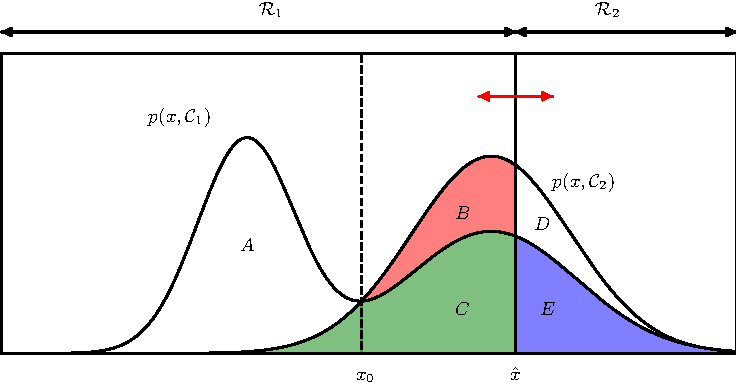
\includegraphics[width=0.7\textwidth]{Figure_10.pdf}
    \end{figure}
\end{frame}

\begin{frame}
    \frametitle{ROC curve}
    \begin{figure}
        \caption{The ROC (receiver operating characteristic) curve}
        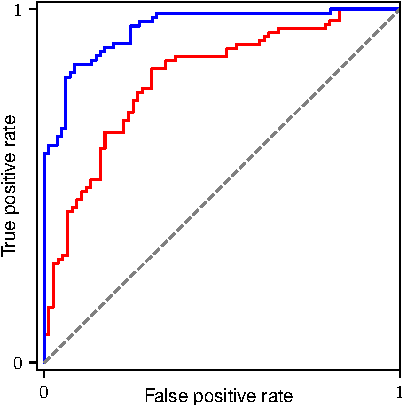
\includegraphics[height=0.7\textheight]{Figure_11.pdf}
    \end{figure}
\end{frame}

\begin{frame}
    \frametitle{ROC curve}
    Some observations:
    \begin{itemize}
        \item The bottom left corner represents a classifier that always outputs negative.
        \item The top left corner represents the best possible classifier.
        \item The top right corner represents a classifier that always outputs positive.
        \item The diagonal line represents a simple random classifier.
    \end{itemize}
    Sometimes it is useful to have a single number that characterises the whole ROC curve:
    \begin{itemize}
        \item The AUC (area under the curve):
        \begin{itemize}
            \item $0.5$: Random guessing.
            \item $1.0$: Perfect classifier.
        \end{itemize}
        \item The F-score: $F=\frac{2\times\textrm{precision}\times\textrm{recall}}{\textrm{precision}+\textrm{recall}}=\frac{2N_{TP}}{2N_{TP}+N_{FP}+N_{FN}}$.
    \end{itemize}
\end{frame}

\section{Generative Classifiers}

\begin{frame}
    \frametitle{Activation functions}
    In linear regression, the model prediction is given by:
    \begin{equation*}
        y(x;w)=w^{T}x+w_{0}
    \end{equation*}
    which gives a continuous-valued output in the range $(-\infty,+\infty)$. For classification problems, we wish to predict posterior probabilities in the range $(0,1)$, which could be achieved using an activation function:
    \begin{equation*}
        y(x;w)=f(w^{T}x+w_{0})
    \end{equation*}
    We see that the decision surfaces are linear functions of $x$. For this reason, these models are called generalized linear models.
\end{frame}

\begin{frame}
    \frametitle{Activation functions}
    For two classes, we can use the logistic sigmoid function $\sigma(a)=\frac{1}{1+\exp(-a)}$ as the activation function:
    \begin{equation*}
        p(\mathcal{C}_{1}|x)=\sigma(a(x))=\frac{1}{1+\exp(-a(x))}
    \end{equation*}
    Compare with:
    \begin{align*}
        p(\mathcal{C}_{1}|x)&=\frac{p(x|\mathcal{C}_{1})p(\mathcal{C}_{1})}{p(x|\mathcal{C}_{1})p(\mathcal{C}_{1})+p(x|\mathcal{C}_{2})p(\mathcal{C}_{2})} \\
        &=\frac{1}{1+\frac{p(x|\mathcal{C}_{2})p(\mathcal{C}_{2})}{p(x|\mathcal{C}_{1})p(\mathcal{C}_{1})}}
    \end{align*}
    We see that:
    \begin{equation*}
        a(x)=\log\frac{p(x|\mathcal{C}_{1})p(\mathcal{C}_{1})}{p(x|\mathcal{C}_{2})p(\mathcal{C}_{2})}
    \end{equation*}
\end{frame}

\begin{frame}
    \frametitle{Activation functions}
    The softmax function is defined by:
    \begin{equation*}
        \mathrm{softmax}(a)=\frac{1}{\sum_{k=1}^{K}\exp(a_{k})}\begin{pmatrix}
            \exp(a_{1}) \\
            \vdots \\
            \exp(a_{K})
        \end{pmatrix}
    \end{equation*}
    For multiple classes, we can use the softmax function as the activation function:
    \begin{equation*}
        \begin{pmatrix}
            p(\mathcal{C}_{1}|x) \\
            \vdots \\
            p(\mathcal{C}_{K}|x)
        \end{pmatrix}
        =\mathrm{softmax}(a_{1}(x),\hdots,a_{K}(x))
    \end{equation*}
    Compare with:
    \begin{equation*}
        p(\mathcal{C}_{k}|x)=\frac{p(x|\mathcal{C}_{k})p(\mathcal{C}_{k})}{\sum_{j}p(x|\mathcal{C}_{j})p(\mathcal{C}_{j})}
    \end{equation*}
    We see that:
    \begin{equation*}
        a_{k}(x)=\log(p(x|\mathcal{C}_{k})p(\mathcal{C}_{k}))
    \end{equation*}
\end{frame}

\begin{frame}
    \frametitle{Continuous inputs}
    Let's assume that the class-conditional densities are Guassian. To start with, we will assume that all classes share the same covariance matrix $\Sigma$:
    \begin{equation*}
        p(x|\mathcal{C}_{k})=\frac{1}{(2\pi)^{\frac{D}{2}}(\det\Sigma)^{\frac{1}{2}}}\exp(-\frac{1}{2}(x-\mu_{k})^{T}\Sigma^{-1}(x-\mu_{k}))
    \end{equation*}
    We will see that this lead to generalized linear models.
\end{frame}

\begin{frame}
    \frametitle{Continuous inputs}
    For two classes:
    \begin{equation*}
        p(\mathcal{C}_{1}|x)=\sigma(a(x))
    \end{equation*}
    where:
    \begin{align*}
        a(x)&=w^{T}x+w_{0} \\
        w&=\Sigma^{-1}(\mu_{1}-\mu_{2}) \\
        w_{0}&=-\frac{1}{2}\mu_{1}^{T}\Sigma^{-1}\mu_{1}+\frac{1}{2}\mu_{2}^{T}\Sigma^{-1}\mu_{2}+\log\frac{p(\mathcal{C}_{1})}{p(\mathcal{C}_{2})}
    \end{align*}
\end{frame}

\begin{frame}
    \frametitle{Continuous inputs}
    For multiple classes:
    \begin{equation*}
        \begin{pmatrix}
            p(\mathcal{C}_{1}|x) \\
            \vdots \\
            p(\mathcal{C}_{K}|x)
        \end{pmatrix}
        =\mathrm{softmax}(a_{1}(x),\hdots,a_{K}(x))
    \end{equation*}
    where:
    \begin{align*}
        a_{k}(x)&=w_{k}^{T}x+w_{k0} \\
        w_{k}&=\Sigma^{-1}\mu_{k} \\
        w_{k0}&=-\frac{1}{2}\mu_{k}^{T}\Sigma^{-1}\mu_{k}+\log{}p(\mathcal{C}_{k})
    \end{align*}
\end{frame}

\begin{frame}
    \frametitle{Maximum likelihood solution}
    \begin{itemize}
        \item There are $N$ input data: $x^{1},\hdots,x^{N}$, where $x^{n}\in\mathbb{R}^{D}$.
        \item There are $N$ target data: $t^{1},\hdots,t^{N}$ using a $1$-of-$K$ binary coding scheme, thus $t^{n}\in\mathbb{R}^{K}$.
        \item The total number of data points in class $\mathcal{C}_{k}$ is denoted by $N_{k}$.
        \item Prior class probabilities are denoted by $\pi_{k}=p(\mathcal{C}_{k})$.
        \item Class-conditional densities are Gaussian: $p(x|\mathcal{C}_{k})=\mathcal{N}(x;\mu_{k},\Sigma)$.
    \end{itemize}
\end{frame}

\begin{frame}
    \frametitle{Maximum likelihood solution}
    \begin{align*}
        p(t^{n}|x^{n})&=\prod_{k=1}^{K}p(\mathcal{C}_{k}|x^{n})^{t^{n}_{k}}=\prod_{k=1}^{K}(\frac{p(x^{n}|\mathcal{C}_{k})\pi_{k}}{p(x^{n})})^{t^{n}_{k}} \\
        &=\frac{1}{p(x^{n})}\prod_{k=1}^{K}\pi_{k}^{t^{n}_{k}}\prod_{k=1}^{K}\mathcal{N}(x^{n};\mu_{k},\Sigma)^{t^{n}_{k}} \\
        -\log{}p(t^{n}|x^{n})&=-\sum_{k=1}^{K}t^{n}_{k}\log\pi_{k} \\
        &+\frac{1}{2}\log\det\Sigma+\frac{1}{2}\sum_{k=1}^{K}t^{n}_{k}(x^{n}-\mu_{k})^{T}\Sigma^{-1}(x^{n}-\mu_{k}) \\
        &+\log{}p(x^{n})+\frac{D}{2}\log{}2\pi
    \end{align*}
\end{frame}

\begin{frame}
    \frametitle{Maximum likelihood solution}
    \begin{align*}
        L&=-\log{}p(t^{1},\hdots,t^{N}|x^{1},\hdots,x^{N})=-\sum_{n=1}^{N}\log{}p(t^{n}|x^{n}) \\
        &=-\sum_{k=1}^{K}N_{k}\log\pi_{k} \\
        &+\frac{N}{2}\log\det\Sigma+\frac{1}{2}\sum_{k=1}^{K}\sum_{n=1}^{N}t^{n}_{k}(x^{n}-\mu_{k})^{T}\Sigma^{-1}(x^{n}-\mu_{k}) \\
        &+\sum_{n=1}^{N}\log{}p(x^{n})+\frac{ND}{2}\log{}2\pi
    \end{align*}
\end{frame}

\begin{frame}
    \frametitle{Maximum likelihood solution}
    \begin{align*}
        \frac{\partial{}L}{\partial\pi_{k}}&=\frac{N_{K}}{\pi_{K}}-\frac{N_{k}}{\pi_{k}}\qquad\pi_{k}=\frac{N_{k}}{N} \\
        \frac{\partial{}L}{\partial\mu_{k}}&=(N_{k}\mu_{k}-\sum_{x^{n}\in\mathcal{C}^{k}}x^{n})^{T}\Sigma^{-1}\qquad\mu_{k}=\frac{1}{N_{k}}\sum_{x^{n}\in\mathcal{C}_{k}}x^{n} \\
        \frac{\partial{}L}{\partial\Lambda}(\Lambda)H&=\frac{1}{2}\mathrm{tr}((\sum_{k=1}^{K}\sum_{x^{n}\in\mathcal{C}_{k}}(x^{n}-\mu_{k})(x^{n}-\mu_{k})^{T}-N\Sigma)H) \\
        \Sigma&=\sum_{k=1}^{K}\frac{N_{k}}{N}S_{k}\qquad{}S_{k}=\frac{1}{N_{k}}\sum_{x^{n}\in\mathcal{C}_{k}}(x^{n}-\mu_{k})(x^{n}-\mu_{k})^{T}
    \end{align*}
\end{frame}

\begin{frame}
    \frametitle{Discrete features}
    Suppose $x\in\mathbb{R}^{D}$ is a feature vector, where each feature $x_{d}\in\{0,1\}$. And further suppose that the different features are independent when conditioned on the class $\mathcal{C}_{k}$. So we have:
    \begin{equation*}
        p(x|\mathcal{C}_{k})=\prod_{d=1}^{D}p(x_{d}|\mathcal{C}_{k})=\prod_{d=1}^{D}\mu_{dk}^{x_{d}}(1-\mu_{dk})^{1-x_{d}}
    \end{equation*}
    Using a softmax activation function, we see that:
    \begin{equation*}
        a_{k}(x)=\sum_{d=1}^{D}(x_{d}\log\mu_{dk}+(1-x_{d})\log(1-\mu_{dk}))+\log{}p(\mathcal{C}_{k})
    \end{equation*}
    which again are linear functions of the input values $x$.
\end{frame}

\begin{frame}
    \frametitle{Exponential family}
    If the class-conditional densities $p(x|\mathcal{C}_{k})$ are members of the subset of the exponential family of distributions given by:
    \begin{equation*}
        p(x|\mathcal{C}_{k};\lambda_{k},s)=\frac{1}{s}h(\frac{1}{s}x)g(\lambda_{k})\exp(\frac{1}{s}\lambda_{k}^{T}x)
    \end{equation*}
    the resulting model will be a generalized linear model. For two classes using the logistic sigmoid activation function:
    \begin{equation*}
        a(x)=\frac{1}{s}(\lambda_{1}-\lambda_{2})^{T}x+\log\frac{g(\lambda_{1})}{g(\lambda_{2})}+\log\frac{p(\mathcal{C}_{1})}{p(\mathcal{C}_{2})}
    \end{equation*}
    For multiple classes using the softmax activation function:
    \begin{equation*}
        a_{k}(x)=\frac{1}{s}\lambda_{k}^{T}x+\log{}g(\lambda_{k})+\log{}p(\mathcal{C}_{k})
    \end{equation*}
\end{frame}

\end{document}